\chapter{identPy: a Software for Parameter Estimation}
\label{ch: Software}

In order to estimate the parameters of mathematical models, such as the one presented on chapter \ref{ch: Models}, a python library called \textit{identPy} was developed by the author. \textit{identPy} provides a customizable framework for parameter estimation with built-in mathematical models and estimation methods. 

With this tool, comparison between performance of methods and precision of models can be easily done. Also, users are allowed to customize or create new features to match their needs without having to rewrite the entire framework, reducing time spent on coding. A Graphical User Interface (GUI) was developed as well, providing a simple environment where users can apply the estimation tool without any contact with the code.

The entire library and GUI were written in Python 3, a powerful, simple and fast high-level programming language that has gained large space in various sectors of industry and academy. Its rise is due mainly to the enormous number of libraries and forums developed and maintained by the users. Some examples of libraries used in this project are \textit{numpy} (for scientific computing), \textit{matplotlib} (graph plotting) and \textit{PySide2} (GUI toolkit). Also, python is open-source, not requiring a paid software to code and most of its applications are free.

The following sections describe how the library is organized and illustrate the estimation process using \textit{identPy} GUI.

\section{\textit{identPy} Library}

\textit{identPy} was developed as a python library so users can simply install the package and apply its features as needed. The library, as well as related scripts and files, is hosted on a \href{https://github.com/gnegrelli/identPy}{GitHub repository} and maintained by the author.

The package contains four submodules named \textbf{error}, \textbf{method}, \textbf{model} and \textbf{objects}. Each one of those submodules initialize core python classes developed for this framework. The entire library architecture was conceived in order to allow future contributors to easily work with it and help expand its applications.

The \textbf{error} module comprises the methods used to evaluate the functional error $J(p)$. Currently, only weighted $l^{2}$-norm is implemented.

Inside \textbf{method} module, users will find the estimation methods implemented by the author and used on this study, as well as auxiliary scripts for parameter classification. Also, script containing a Particle Swarm Optimization algorithm implementation can be found in this module.

All classes with mathematical models are organized inside the \textbf{model} module. Besides the WPP equivalent model presented before, this module contains simple models used for testing, such as Spring-Mass and Pendulum systems, and other complex models used in previous studies, such as Linearized Z-IM Load Model. It also has a submodule within that implements implicit methods, such as the Runge-Kutta method, applied to obtain the behaviour of these models.

Finally, the estimator object and all abstract classes developed are organized inside \textbf{objects}. The Estimator object is responsible for building the estimation framework, by gathering the measured data, model and estimation methods, and executing it. The abstract classes located here constitute base objects from where the other classes can inherit.

\section{\textit{identPy} GUI}

The \textit{identPy} GUI was created with \textit{Qt}, a software for design of user interfaces and applications. The views and scripts created specifically for the GUI application are hosted on a different \href{https://github.com/gnegrelli/identPy_GUI}{repository}. When the application is launched, a starting window with information about the software and its development are displayed, as shown in Figure \ref{fig: initial_page}.

\begin{figure}[!h]
	\caption{\textit{identPy} initial page}
	\begin{center}
		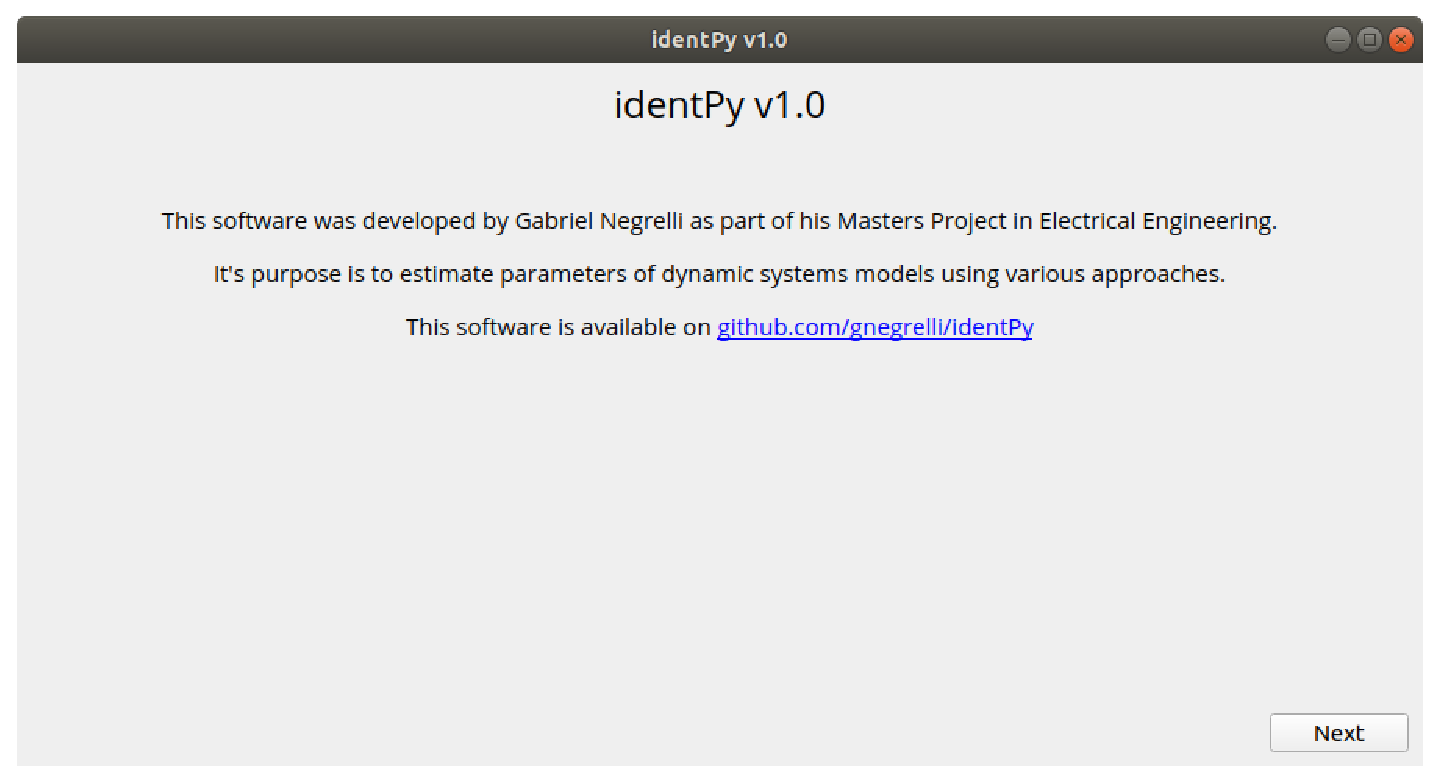
\includegraphics[scale=.5]{Images/Software_initial_page.eps}
	\end{center}
	\label{fig: initial_page}
\end{figure}

Next, a page for model selection is shown. The page layout is depicted in Figure \ref{fig: model_selection}. In this page, the user will choose, from a list indicated by "1", which mathematical model will be estimated. In "2", the user will be able to select the file containing the measured data used in the estimation process. The measured data must be in .csv, .dat or .txt format in order to be read correctly by the software. In the field indicated by "3", the user must identify which column of the data file corresponds to the inputs and outputs and what are initial conditions of states. Notice that the column containing the time measurement must be the first one on the file (indicated by the column index $0$). The area indicated by "4" displays a short text with information about the model selected.

\begin{figure}[!h]
	\caption{Model selection page}
	\begin{center}
		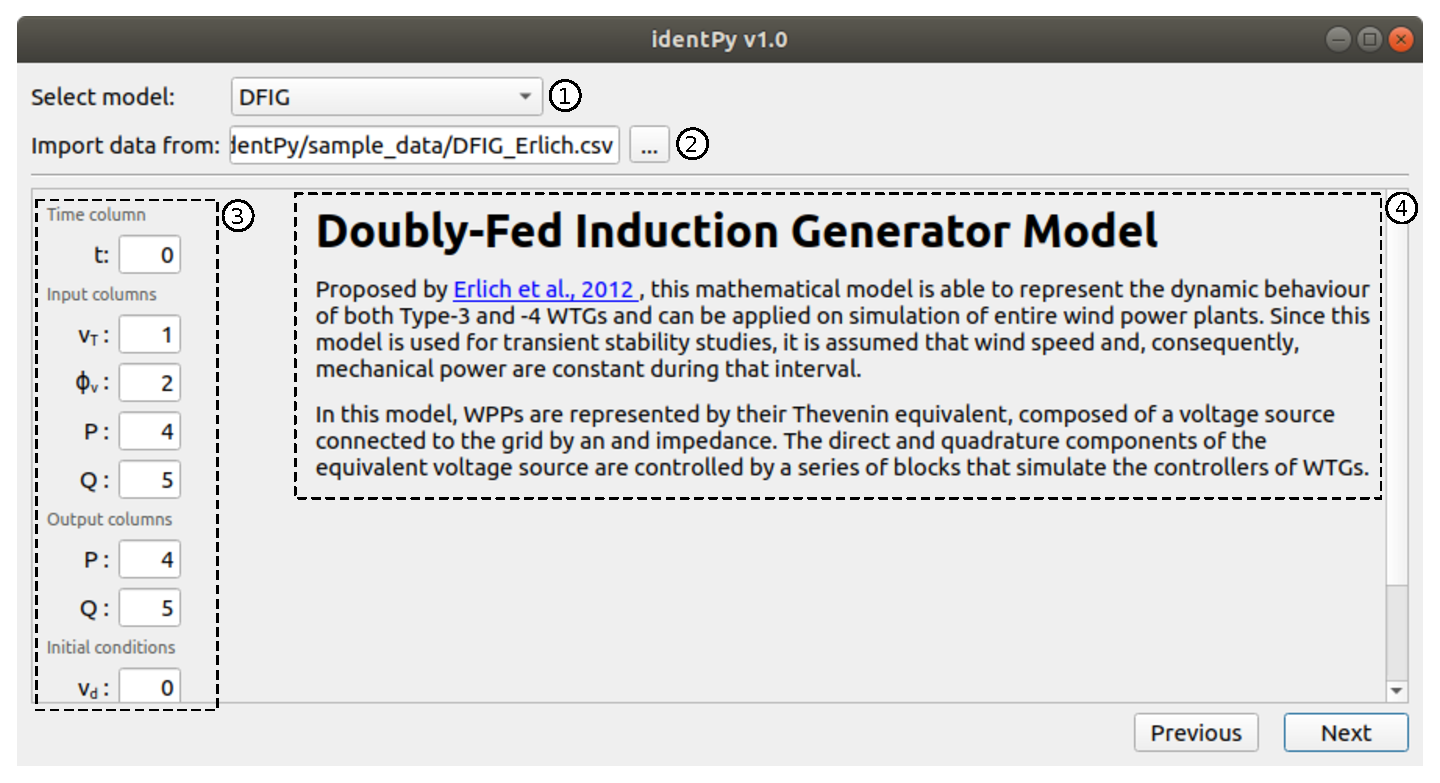
\includegraphics[scale=.5]{Images/Software_model_page.eps}
	\end{center}
	\label{fig: model_selection}
\end{figure}

On the next page, the user will be able to select two estimation methods from the list of available methods, as displayed in Figure \ref{fig: method_selection}. The drop-down list, indicated by "5", contains all methods available for estimation. The method selected in this field will be the first applied by the estimation tool. In "6", the user can indicate that the estimation will be conducted by two methods in cascade, as the hybrid method explained in the previous chapter. The second method to be applied can be selected in "7".

\begin{figure}[!h]
	\caption{Method selection page}
	\begin{center}
		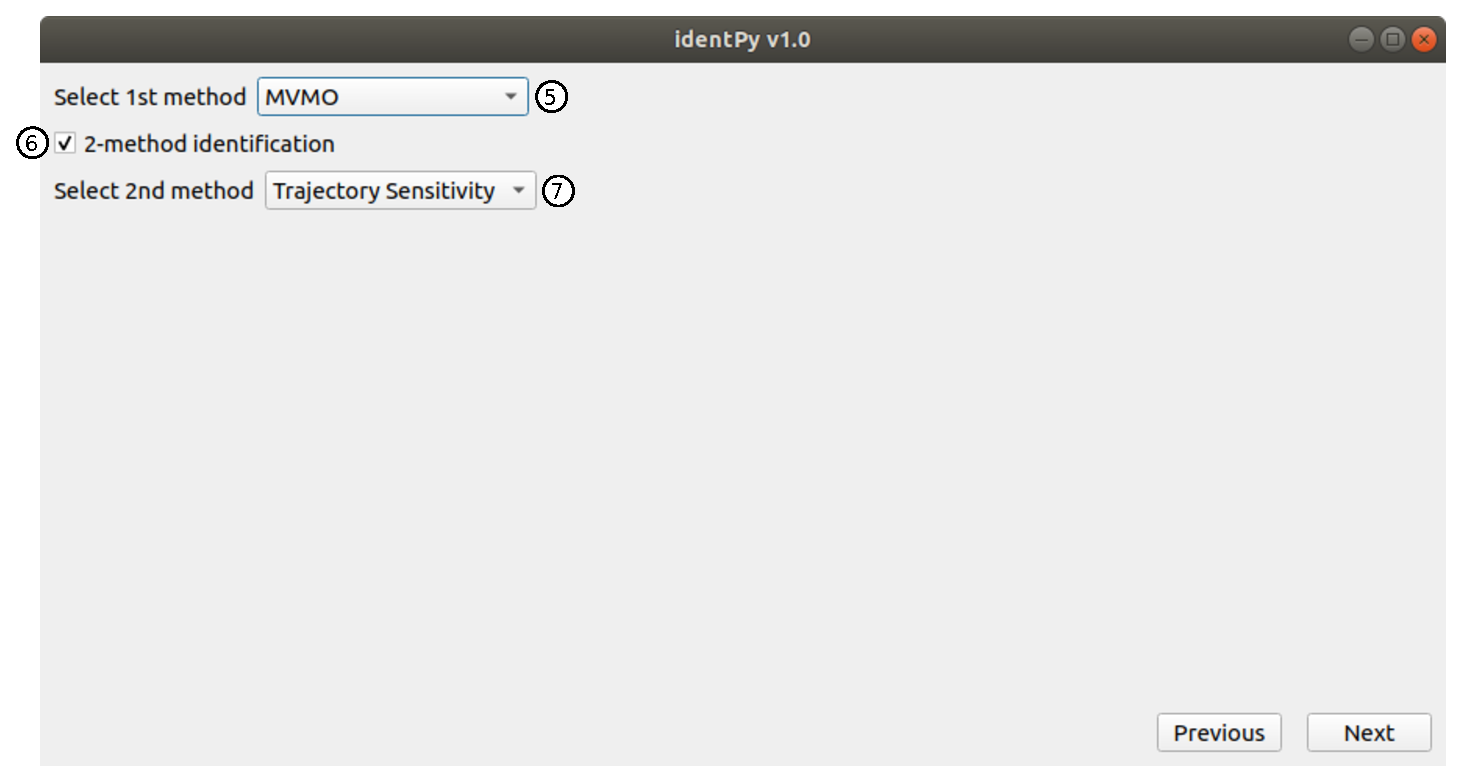
\includegraphics[scale=.5]{Images/Software_method_page.eps}
	\end{center}
	\label{fig: method_selection}
\end{figure}

The configuration of the chosen methods is done on the following windows. Each method has its own custom configuration page based on a template.

MVMO configuration page is depicted in Figure \ref{fig: MVMO_page}. For this method, the user must set general configurations, such as population size, number of offspring and tolerance. These general configurations are set on the fields indicated by "8". The user must also define what are the limits of the search region, which are set on the fields identified by "9". These fields change according to the choice made by the user on the model selection page.

\begin{figure}[!h]
	\caption{MVMO configuration page}
	\begin{center}
		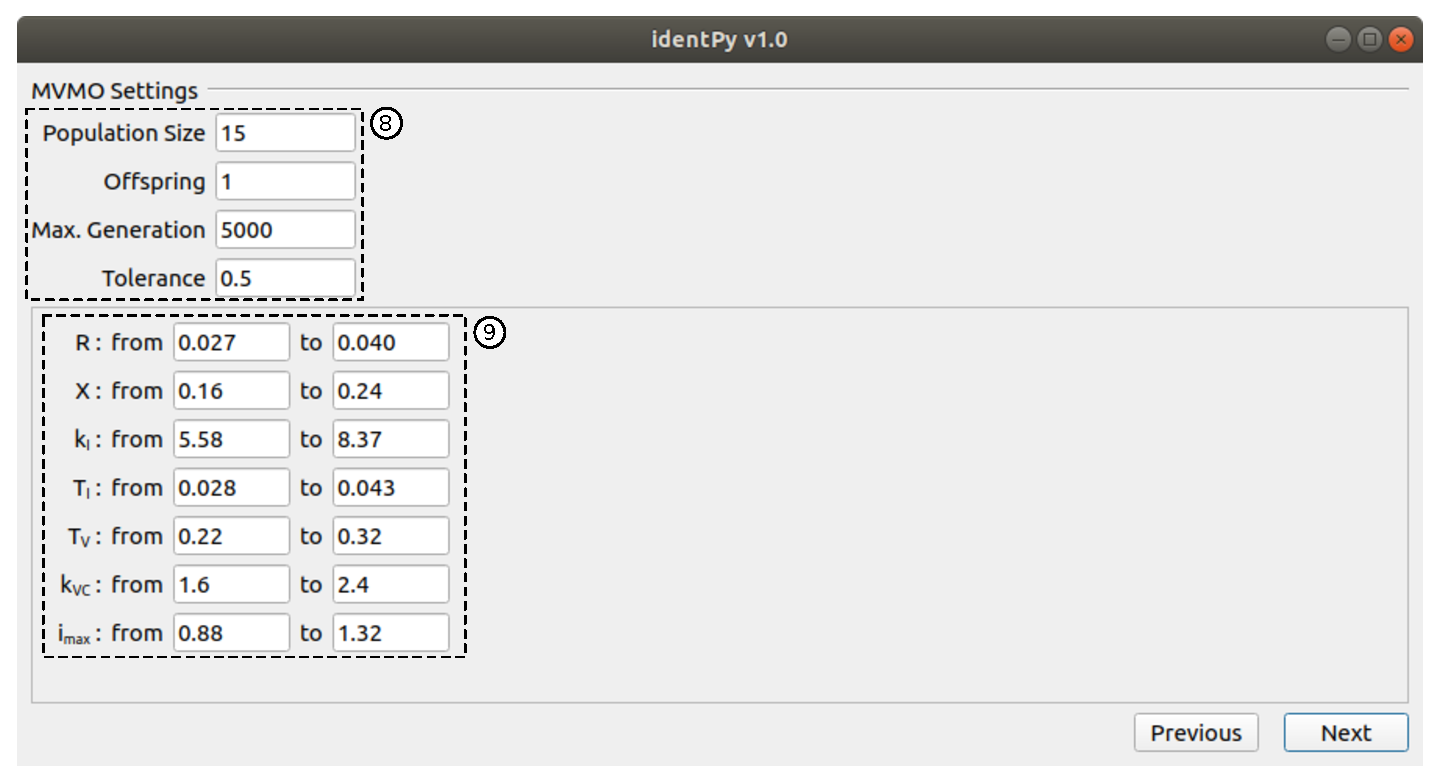
\includegraphics[scale=.5]{Images/Software_MVMO_page.eps}
	\end{center}
	\label{fig: MVMO_page}
\end{figure}

The configuration page of TSM, shown in Figure \ref{fig: TS_page}, is relatively similar to the MVMO page. General configurations (number of iterations and tolerance) are set in "10". The initial values of the parameters used as starting point by TSM are set in "11". If this is the second method of a hybrid approach, the initial values will be the ones found by the previous method. In this case, the values entered in "11" will be discarded by the software.

\begin{figure}[!h]
	\caption{TSM configuration page}
	\begin{center}
		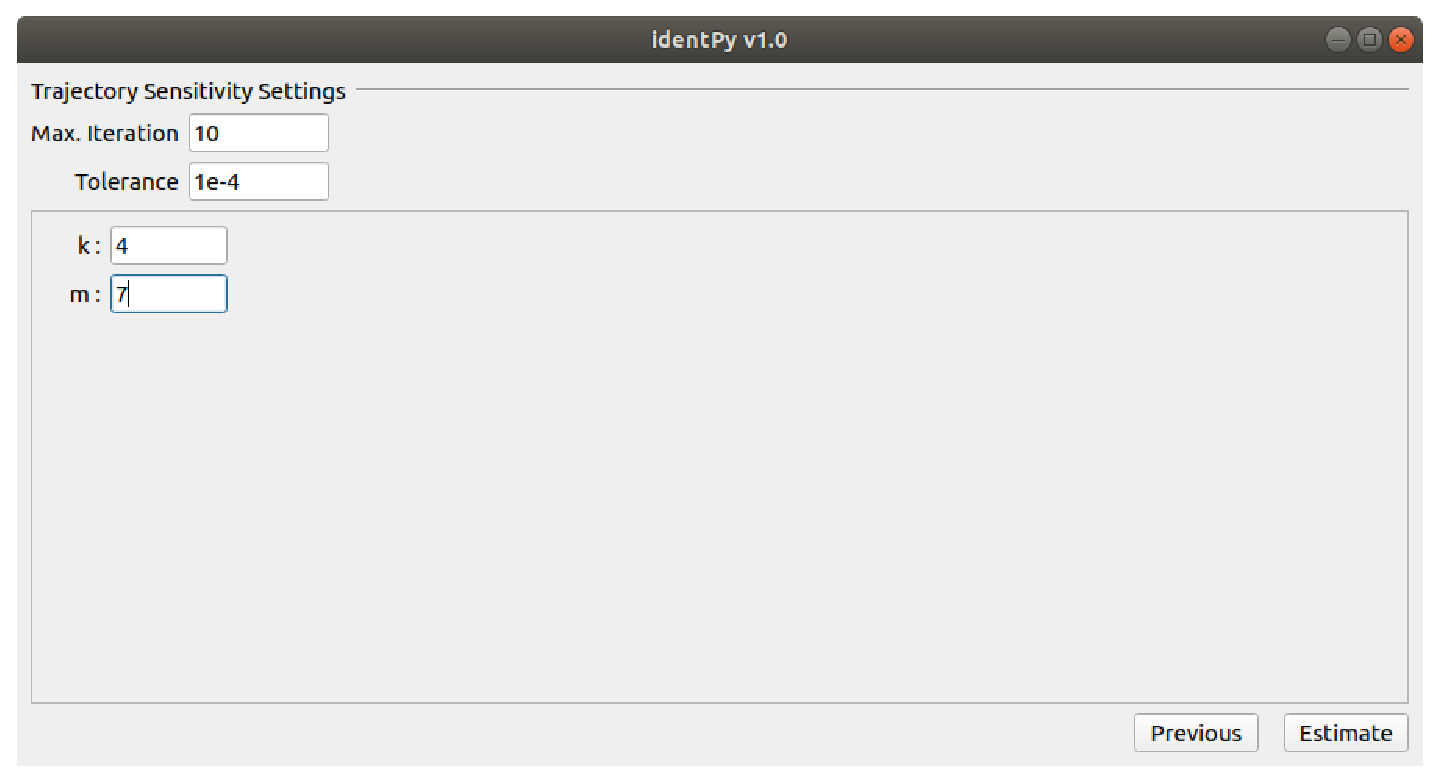
\includegraphics[scale=.5]{Images/Software_TS_page.eps}
	\end{center}
	\label{fig: TS_page}
\end{figure}

With all set, the estimation process can now start. The page depicted in Figure \ref{fig: final_pg} is displayed to the user while the estimation runs on background.

\begin{figure}[h]
	\caption{Results page}
	\begin{center}
		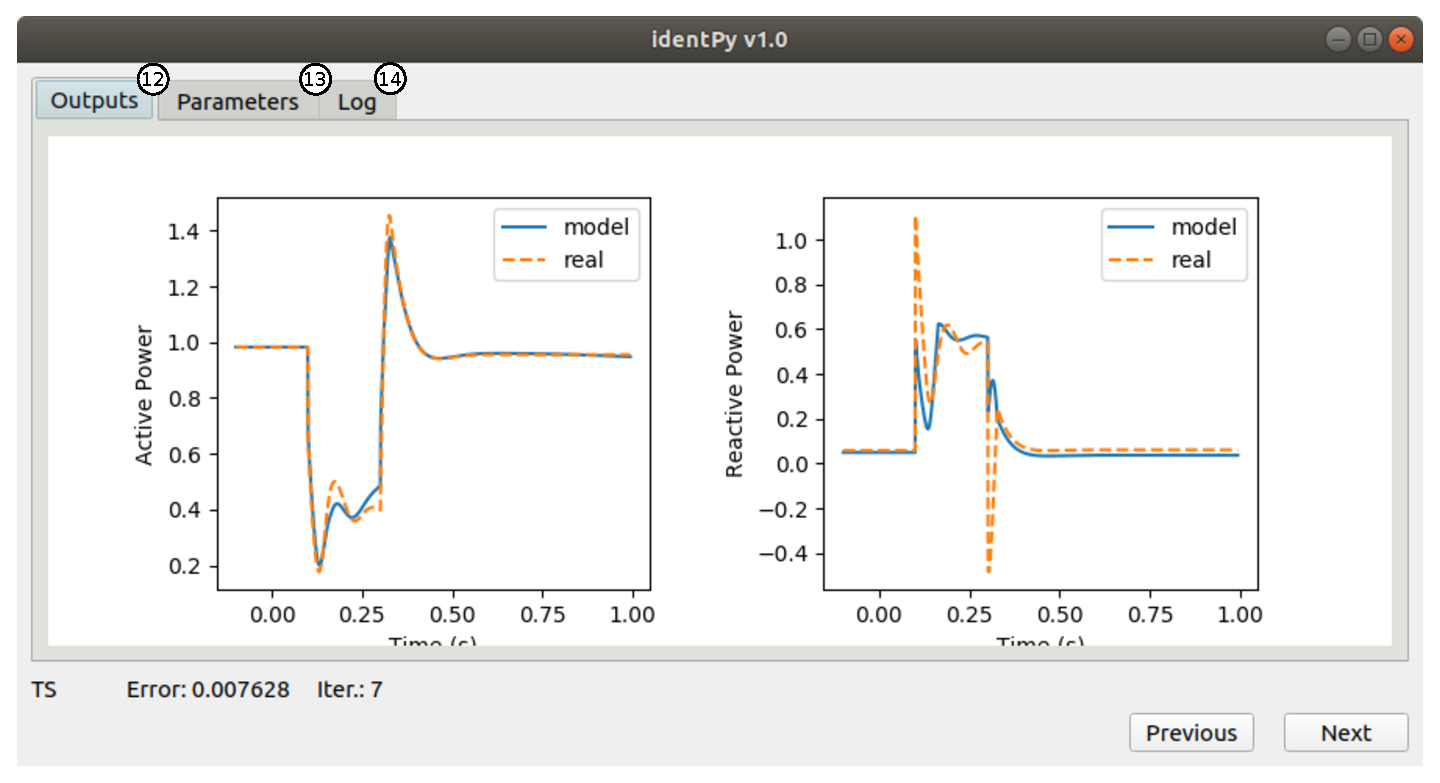
\includegraphics[scale=.5]{Images/Software_results_page.eps}
	\end{center}
	\label{fig: final_pg}
\end{figure}

On the tab indicated by "12", graphs depicting the outputs from the real system and the current solution are shown. The tab identified by "13" presents the current value of the parameters estimated by the software. A log with information of how the estimation process evolved is displayed in "14". The data shown in those three tabs are updated as the estimation process runs, with all information representing the current solution found.

As the estimation package evolves, other pages may be included in order to improve the software performance. For instance, as the methods list grows, configuration pages will be designed to set these new methods. Also, a page to analyze model identifiability may be included to enhance the estimation software.